
%!TEX ROOT=ctutest.tex

\chapter{Rešerše}


\section{Podlahové topení}

U podlahového vytápění dochází k přenosu tepla do vytápěného prostoru převážně sáláním. Což má za následek, že se od sálající plochy ohřívají plochy osálané a teprve od sálajících a osálaných ploch se ohřívá okolní vzduch (druhá konvenkční složka z celkového tepelného toku). Naproti tomu při přenosu tepla pomocí tradičních radiátorů dochází k přenosu pomocí proudění (konvekční složka). 
Teplota otopné plochy je poměrně nízká pohybuje se mezi 25 až 34 °C u podlahového vytápění a tedy i teplota teplonosné látky je nízká (otopná plocha je zahřívaná buď teplou vodou, teplým vzduchem nebo elektricky). Proto je tento typ vytápění vhodné využít při zapojení s nízkoteplotním zdrojem, jako jsou tepelná čerpadla, kondenzační kotle či solární panely.

Důležitým parametrem pro příjemný pobyt v místnosti je prostorové rozložení teploty, jak ve vertikální tak horizontální rovině. Na vertikální rozložení teplot ve vytápěné místnosti je způsobeno nerovnoměrným přívodem tepla a nerovnoměrným ochlazování jednotlivých stěn místnosti. Vertikální nerovnoměrnost teplot je tím větší, čím vyšší je povrchová teplota otopné plochy. Vzhledem k tomu, že teplota u podlahové vytápění je povrchová teplota otopné vody ze všech druhů velkoplošného vytápění (podlahové, stropní, stěnové) nejnižší, je vertikální rozložení teplot skoro ideální. Co se týče rozložení teplot v jednotlivých vrstvách místnosti, je teplota v úrovni hlavy maximálně o 2 až 3 °C vyšší než v oblasti kotníků a směrem od zóny pobytu již klesá. V porovnání s ostatními druhy vytápění je vertikální průběh teplot značně nerovnoměrný. Optimální vytápění by mělo zajistit, aby v oblasti hlavy stojícího člověka byla teplota minimálně o 2 °C nižší než je v úrovni kotníků. Takovému ideálnímu průběhu (obrázek  \ref{fig:vertikalni-prubehy-teplot-pro-ruzne-druhy-vytapeni}a) teplot odpovídá obrázek \ref{fig:vertikalni-prubehy-teplot-pro-ruzne-druhy-vytapeni}b. Dále jsou na obrázku  \ref{fig:vertikalni-prubehy-teplot-pro-ruzne-druhy-vytapeni} jsou další druhy vytápění s vertikálními průběhy teplot. Na obrázku \ref{fig:porovnani-rozlozeni-teplot} je prostorové porovnání teplot podlahové vytápění a vytápění při využití radiátorů s vyznačenými oblastmi teplot.


\begin{figure}[H]

\centering
\begin{picture}(370,70)
\put(0,0){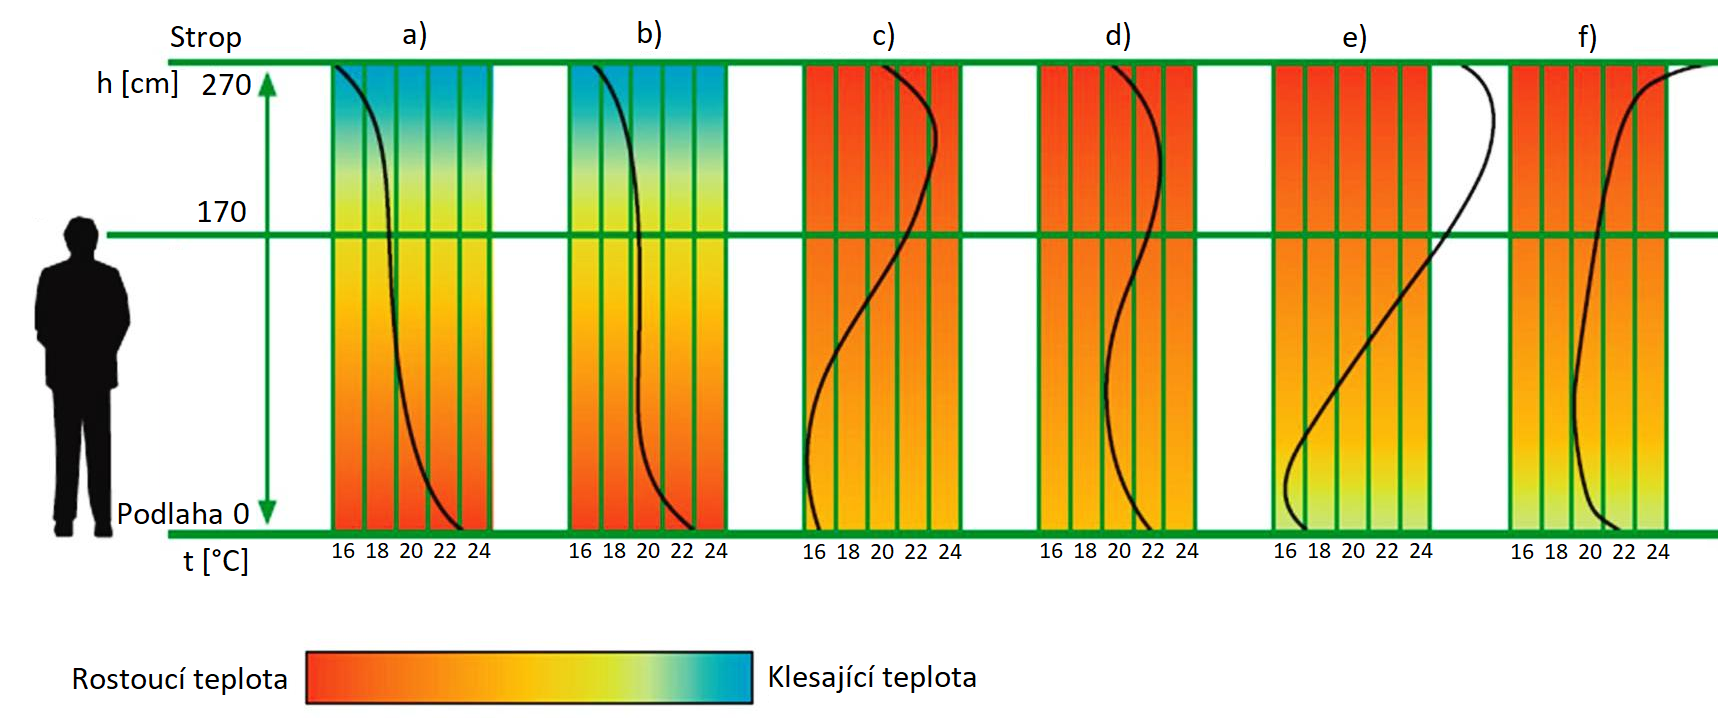
\includegraphics[width=\textwidth]{images/vertikalni-prubehy-teplot-pro-ruzne-druhy-vytapeni.png}}
\put(5,6){\scriptsize \sffamily Rostoucí teplota}
\put(161,6){\scriptsize \sffamily Klesající teplota}
\put(19,31){\scriptsize \sffamily t[°C]}
\put(15,132){\scriptsize \sffamily h[cm]}
\put(22,41){\fontsize{6}{6} \sffamily Podlaha}
\put(22,141){\fontsize{6}{6} \sffamily Strop}
\put(50,41){\scriptsize \sffamily 0}
\put(40,104){\scriptsize \sffamily 170}
\put(40,132){\scriptsize \sffamily 270}

\put(84,143){\scriptsize \sffamily a)}
\put(67,33){\fontsize{5}{5} \sffamily 16}
\put(74,33){\fontsize{5}{5} \sffamily 18}
\put(81,33){\fontsize{5}{5} \sffamily 20}
\put(88,33){\fontsize{5}{5} \sffamily 22}
\put(95,33){\fontsize{5}{5} \sffamily 24}

\put(134,143){\scriptsize \sffamily b)}
\put(117,33){\fontsize{5}{5} \sffamily 16}
\put(124,33){\fontsize{5}{5} \sffamily 18}
\put(131,33){\fontsize{5}{5} \sffamily 20}
\put(138,33){\fontsize{5}{5} \sffamily 22}
\put(145,33){\fontsize{5}{5} \sffamily 24}

\put(184,143){\scriptsize \sffamily c)}
\put(167,33){\fontsize{5}{5} \sffamily 16}
\put(174,33){\fontsize{5}{5} \sffamily 18}
\put(181,33){\fontsize{5}{5} \sffamily 20}
\put(188,33){\fontsize{5}{5} \sffamily 22}
\put(195,33){\fontsize{5}{5} \sffamily 24}

\put(234,143){\scriptsize \sffamily d)}
\put(217,33){\fontsize{5}{5} \sffamily 16}
\put(224,33){\fontsize{5}{5} \sffamily 18}
\put(231,33){\fontsize{5}{5} \sffamily 20}
\put(238,33){\fontsize{5}{5} \sffamily 22}
\put(245,33){\fontsize{5}{5} \sffamily 24}

\put(284,143){\scriptsize \sffamily e)}
\put(267,33){\fontsize{5}{5} \sffamily 16}
\put(274,33){\fontsize{5}{5} \sffamily 18}
\put(281,33){\fontsize{5}{5} \sffamily 20}
\put(288,33){\fontsize{5}{5} \sffamily 22}
\put(295,33){\fontsize{5}{5} \sffamily 24}

\put(334,143){\scriptsize \sffamily f)}
\put(317,33){\fontsize{5}{5} \sffamily 16}
\put(324,33){\fontsize{5}{5} \sffamily 18}
\put(331,33){\fontsize{5}{5} \sffamily 20}
\put(338,33){\fontsize{5}{5} \sffamily 22}
\put(345,33){\fontsize{5}{5} \sffamily 24}
\end{picture}
	 \caption{Vertikální průběh teploty vzduchu ve vytápěné místnosti při různém způsobu vytápění. Upraveno z \cite{vertikalni-prubehy-teplot-pro-ruzne-druhy-vytapeni}. \\ a) Ideální požadovaný průběh, b) Podlahové vytápění, c) Vytápění radiátory (vnitřní stěna), d) Vytápění radiátory (venkovní stěna), e) Teplovzdušné vytápění (podlahové konvektory), f) Stropní vytápění }
	 \label{fig:vertikalni-prubehy-teplot-pro-ruzne-druhy-vytapeni}
\end{figure}

\hspace{5mm}

  \begin{figure}[H]
     \subfloat[Rozložení teplot při použití podlahové topení.\label{fig:rozlozeni-teplot-podlahove-vytapeni}]{
       \begin{overpic}[width=0.5\textwidth]{images/rozlozeni-teplot-podlahove-vytapeni.png}
         \put(20,10){\scriptsize \sffamily 22 °C}
         \put(65,50){\scriptsize \sffamily 20 °C}
         \put(8,115){\scriptsize \sffamily 17 °C}
         \put(155,90){\scriptsize \sffamily 18 °C}
       \end{overpic}
     }
     \subfloat[Rozložení teplot při použití radiátorů. \label{fig:rozlozeni-teplot-radiatory}]{
       \begin{overpic}[width=0.5\textwidth]{images/rozlozeni-teplot-radiatory.png}
         \put(20,10){\scriptsize \sffamily 14 °C}
         \put(100,15){\scriptsize \sffamily 33 °C}
         \put(133,37){\scriptsize \sffamily 37 °C}
         \put(32,50){\scriptsize \sffamily 22 °C}
         \put(113,77){\scriptsize \sffamily 30 °C}
         \put(20,87){\scriptsize \sffamily 19 °C}
         \put(160,95){\scriptsize \sffamily 20 °C}
         \put(42,117){\scriptsize \sffamily 23 °C}
       \end{overpic}
     }
     \caption{Porovnání rozložení teplot při použití podlahové topení a radiátorů. Upraveno z \cite{rozlozeni-teplot-podlahove-vytapeni-a-radiatory}.}\label{fig:porovnani-rozlozeni-teplot}
   \end{figure}
   


\subsubsection{Výhody}

\begin{itemize}
  \item Je vhodné zejména tam, kde je nízkoteplotní zdroj tepla (tepelné čerpadlo, kondenzační kotel, solární panely, …).
  \item Větší užitný prostor (místo nezabírají otopná tělesa).
  \item Cirkulace vzduchu je nižší oproti radiátorům, proto je víření prachu v místnosti menší.
  \item Téměř rovnoměrná teplota místnosti.
\end{itemize}

\subsubsection{Nevýhody}

\begin{itemize}
  \item Zvýšené náklady na realizaci.
  \item Nezbytná pečlivá montáž a stavební dozor.
  \item Vyšší tepelná setrvačnost otopné soustavy.
  \item Vyšší nároky na řízení podlahové otopné plochy (zejména hlídání maximální vstupní otopné vody).
\end{itemize}


\section{Zónová regulace vytápění}

Význam zónové regulace spočívá v systému umožňující individuální vytápění v jednotlivých místnostech (každá místnost nebo spojení více místností označuje zónu) na požadovanou teplotu.  Základ zónové regulace je centrální řídící jednotka, která přijímá data od jednotlivých místností (zejména jejich aktuální teplotu) a dává povely na zařízení, které ovládá (otevírání/zavírání pohonů u jednotlivých otopných těles apod.). Přístup k řídící jednotce je nejčastěji pomocí displeje, webového rozhraní nebo jejich kombinace. V řídíc jednotce se dá celý systém vytápění nastavit (nastavení časových a teplotních programu pro jednotlivé zóny a mnohé další). 

Zónové systémy vytápění se rozdělují na dvě hlavní skupiny. První tvoří zónové systémy propojené pomocí vodičů. Druhou skupinu tvoří bezdrátová technologie propojující řídící jednotkou a jednotlivé zóny. 

Hlavní částí zónového systému je centrální řídící jednotka. Mezi další komponenty patří: nástěnné snímače vnitřní teploty, snímač venkovní teploty, termoelektrické pohony, elektronické regulátory otopných těles, reléová spínací jednotka. Mezi komponenty, které přispívají ke komfortu zónové regulace patří: senzor intenzity slunečního záření, senzor rychlosti větru, různé spínací jednotky, jednotky pro ovládání žaluzií, moduly pro dálkové ovládání pomocí GSM a další.
\subsection{Principy zónové regulace}
Jak již bylo řečeno, základem celého systému je centrální řídicí jednotka. Další důležitou komponentou je zónový regulátor, který slouží pro ovládání komponent, které jsou k zónovému regulátoru připojeny. Mezi hlavní komponenty, který zónový regulátor ovládá jsou termoelektrické pohony. Termoelektrický pohon je podobný termostatické hlavici, která se nasazuje na radiátorový ventil, ale je jej možné ovládat elektrickým napětím. Samotná regulace vytápění probíhá tak, že řídící jednotka je propojena se zónovým regulátorem. K zónovému regulátoru jsou připojeny jednotlivé nástěnné snímače  prostorové teploty a termoelektrické pohony, které jsou nasazeny na termostatický ventilech otopných okruhů/těles. V řídící jednotce jsou nastaveny časové programy (různé požadované teploty pro různé časové úseky). Řídíc jednotka posílá do zónového regulátoru požadované teploty pro všechny zóny. Tyto  teploty jsou v zónovém regulátoru porovnávány s aktuálními prostorovými teplotami měřenými nástěnnými jednotkami. V případě, že je prostorová teplota příslušné zóny nižší než požadovaná teplota (nastavená v řídicí jednotce), ovládá zónový regulátor odpovídající pohon, který otevírá/zavírá daný ventil a umožňuje proudění otopné vody do otopného okruhu/tělesa, čím dochází ke změny teploty v místnosti. Pokud je připojen například kotel, je pak hořák kotle ovládán při požadavku vytápění v jakékoliv místnosti. 

Další možné zapojení může být takové, že jednotlivé nástěnné snímače prostorové teploty jsou přímo propojeny s řídící jednotkou, která následně podle časového programu posílá zónovému regulátoru požadavky na ovládání jednotlivých pohonů. 

Mezi další ovládána zařízení při regulace vytápění mohou být čerpadla, směšovací ventily zejména pro podlahové vytápění, kde je nutné udržovat teplotu otopné vody v daných mezích.

DOPLNIT OBRAZEK (vlastni schema)



\subsection{Dostupné komerční/nekomerční řešení zónové regulace podlahového vytápění}
\subsection{PocketHome}
\subsection{Jablotron}
\subsection{Salus}
\subsection{Honeywell Evohome}







